\section{Project 10 - Image Representation and Description}
\subsection{Project Proposal}
There are two parts in project 10. 
\textbf{(a)} Develop a program to implement the boundary following algorithm, the resampling grid and calculate the chain code and the first difference chain code. Use the image 'noisy\_stroke.tif' for test. 
\textbf{(b)} Develop a program to implement the image description by the principal components. Calculate and display the PC images and the reconstructed images from 2 PCs. Use the six images in 'washingtonDC.rar' as the test images.

\subsection{Preliminaries}
\subsubsection{Boundary following}
Given a binary region $R$ or its boundary, an algorithm for following the border of $R$ consists of the following steps:\\
\textbf{1.} Let the starting point $b_0$ be the uppermost, leftmost point in the image that is marked 1. Denote by $c_0$ the west neighbor of $b_0$ which is unmarked. Examine 8-neighbors of $b_0$, starting at $c_0$ and proceeding in clockwise direction. Let $b_1$ denote the first neighbor encountered whose value is 1, and let $c_1$ be the point immediatly preceding $b_1$ in the sequence. Store the locations of $b_0$ and $b_1$ for use in Step 5.\\
\textbf{2.} Let $b=b_1$ and $c=c_1$.\\
\textbf{3.} Let the 8-neighbor of $b$, starting at $c$ and proceeding in a clockwise direction, be denoted by $n_1,...,n_8$. Find the first $n_k$ labeled 1.\\
\textbf{4.} Let $b=n_k$ and $c=n_{k-1}$.\\
\textbf{5.} Repeat Steps 3 and 4 until $b=b_0$ and next boundary point found is $b_1$. The sequence of $b$ points found when the algorithm stops constitutes the set of ordered boundary points.\\
\subsubsection{Chain Codes}
Chain codes are used to represent a boundary by a connected sequence of straight line segments of specified length and direction. The commonly used directions are 4-connectivity or 8-connectivity (Fig.\ref{fig:10direction}). This representation is also referred as \emph{Freeman chain code}.
\begin{figure}[h!]
	\centering
	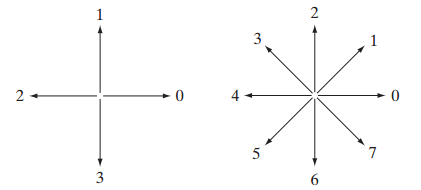
\includegraphics[width=0.45\linewidth]{myfigure/p10/direction.png}
	\caption{left: 4-directional chain code; right: 8-directional chain code.}
	\label{fig:10direction}
\end{figure}
If we directly generate the chain code with the border following method talked above, the chain will be too long and any small disturbances along the boundary will cause changes in the code that may not be related to the principal shape features of the boundary. An frequently used approach to circumvent is to resample the boundary by selecting a larger grid spacing. Resampling means that as the boundary is traversed, a boundary point is assigned to each node of the large grid, depending on the proximity of the original boundary to that node. The chain code is depends on the starting point, but if we regard it as a circular sequence, then the result is independent to the start point. For rotation, we also have a normalization method that replace the original chain code with \emph{first difference} of the chain code. This difference is obtained by counting the number of direction changes that separate two adjacent elements of the code. To convert the difference to circular sequence, we only need to pad one value that satisfy the head and tail values. Size normalization can be achieved by altering the size of the resmapling grid. Hence, chain code is good representation that resistant the geometric transformation - translation, rotation and scaling.

\subsubsection{Use of principle components for description}
If we have $n$ registered images, the vector represents one common pixel in all $n$ images is $\mathbf{x}^T=[x_1, x_2,..., x_n]$. We treat the vectors as random quantities, then mean vector is \begin{equation}\mathbf{m_x}=E[\mathbf{x}]\approx \frac{1}{K}\sum_{k=1}^K\mathbf{x}_k\end{equation} and the covariance matrix is \begin{equation} \mathbf{C_x}=E\left[(\mathbf{(x-m_x)(x-m_x)^T} \right] \approx \frac{1}{K}\sum_{k=1}^K\mathbf{x_kx_k^T-m_xm_x^T}\end{equation}As $\mathbf{C_x}$ is real and symmetric, finding a set of $n$ orthonormal eigenvectors always is possible. Let $\mathbf{A}$ be a matrix whose rows are formed from the eigenvectors of $\mathbf{C_x}$ and the corresponding eigenvalue is descending from top to bottom. Then we define \emph{Hotelling transform} $\mathbf{y=A(x-m_x)}$. There are many interesting properties of $\mathbf{y}$, e.g. as $\mathbf{A}^{-1}=\mathbf{A}^T$, we can recover $\mathbf{x}=\mathbf{A}^T\mathbf{y}+\mathbf{m_x}$. Suppose, however, that instead of using all the eigenvectors of $\mathbf{C_x}$  we form matrix $\mathbf{A}_k$ from the top $k$ eigenvectors. Thus the $\mathbf{y}$ vectors will be $k$ dimensional and the reconstruction is described as $\hat{\mathbf{x}}=\mathbf{A}_K^T\mathbf{y}+\mathbf{m_x}$
